\section{Language Integrated Query (LINQ)}
Ist eine Sprach-Integrierte Abfragesprache.
\begin{itemize}
	\itemsep -0.5em 
	\item Reine Compiler-Technologie
	\item Query-Syntax (ähnlich SQL)
	\item Beliebige Datenstrukturen als Basis (Objekte, XML etc.)
	\item Typensicherheit
	\item Erlaubt funktionale Progammierung mit Lambda
	\item Erlaubt deklarativen Progammierstil mittels Anonymous Types" und Object "initializers"
	\item Verbesserung Type Inference
\end{itemize}

\begin{figure}[h!]
	\centering
	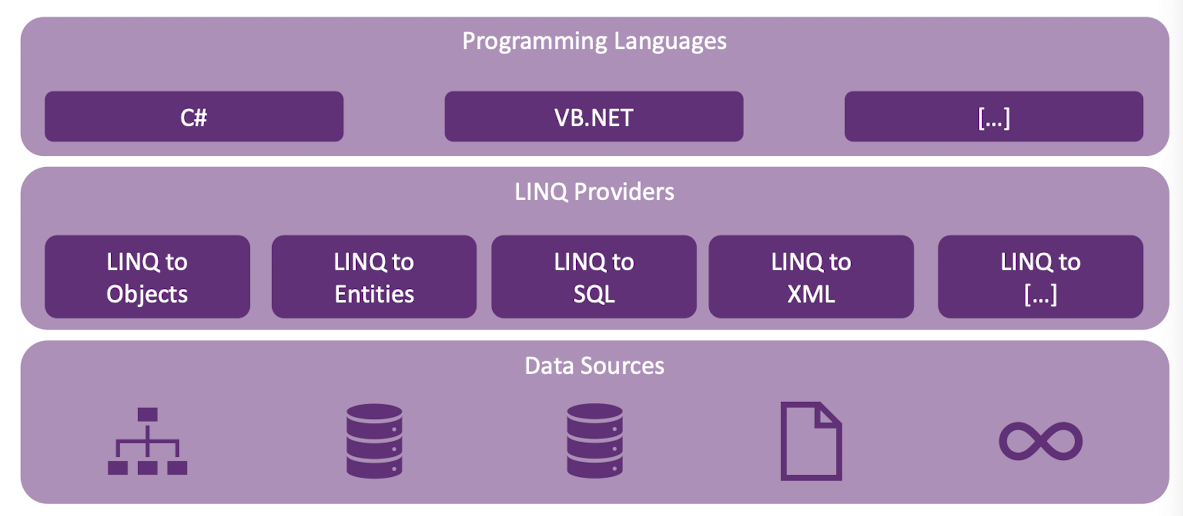
\includegraphics[width=0.5\linewidth]{linq}
  \caption{Die Architektur von LINQ}
\end{figure}


\subsection{LINX Extension Methods}
LINQ definiert in der Klasse Enumerable eine Vielzahl von Query Operatoren. Die Methoden in dieser Klasse stellen eine Implementierung von Operatoren zum Abfragen von Datenquellen bereit, die IEnumerable<T> implementieren. 

\subsection{Expression-Bodies Members}



\subsection{Objection/Collection Initializers}



\subsection{Anonymous Types}




\subsection{Query Expressions}


\pagebreak
